\chapter{Análisis de las herramientas e infraestructuras utilizadas}
\label{cap:analisis}

[Revisar]\\

En este capítulo se realiza un breve análisis de las distintas herramientas e infraestructuras usadas a lo largo del proyecto.


\section{Análisis de la herramienta de virtualización \emph{hardware}}

A la hora de hacer una virtualización \emph{hardware} hay varias opciones entre las que elegir. Las más ampliamente usadas son Xen y KVM. La principal diferencia entre ambas es que Xen ofrece paravirtualización y KVM ofrece virtualización nativa.

La virtualización nativa permite hacer una virtualización \emph{hardware} completa de manera eficiente. No requiere de ninguna modificación en el sistema operativo de la máquina virtual, pero necesita de un procesador con soporte para virtualización. KVM está incluido como un módulo del núcleo de Linux desde su versión 2.6.20, así que viene incluido por defecto en cualquier sistema operativo con núcleo Linux.

Como los ordenadores del laboratorio poseen procesadores con extensiones de soporte para virtualización y sistema opetativo Debian, se eligió KVM para dar soporte a las máquinas virtuales. Esto significa que podemos usar cualquier sistema operativo para las máquinas virtuales, sin necesidad de hacer ninguna modificación.


\section{Análisis de las infraestructuras de ejecución de trabajos distribuidos}

%%% Revisar
AppScale es una implementación \emph{open source} del App Engine de Google. Al igual que App Engine, AppScale permite alojar aplicaciones web; a diferencia de App Engine, las aplicaciones no serán alojadas en la infraestructura que Google posee, sino que serán alojadas en una infraestructura que el usuario posea. Además de permitir alojar aplicaciones web, AppScale también ofrece las APIs de MapReduce y Neptune. La API de MapReduce permite escribir aplicaciones que hagan uso del \emph{framework} MapReduce. La API de Neptune añade a App Engine la capacidad de usar los nodos de la infraestructura para ejecutar trabajos. Los trabajos más representativos que puede ejecutar son: de entrada, de salida y MPI, aunque también se pueden ejecutar trabajos de otro tipo.

Una vez puesta en marcha la infraestructura de AppScale, servirá tanto para alojar las aplicaciones web que el usuario despliegue como para ejecutar trabajos. Para desplegar las aplicaciones web hay que hacer uso de las AppScale Tools, un conjunto de herramientas que permiten, entre otras cosas: iniciar y terminar instancias, desplegar aplicaciones y eliminar aplicaciones. Para ejecutar trabajos hay que servirse de la API de Neptune, que no es tan sencilla. En general esto se consigue mediante tres pasos: en el primero se le indica el código fuente que se quiere subir a la infraestructura; en el segundo se le da la orden de ejecutar el trabajo; en el tercero se le piden los resultados de la ejecución. Cada uno de estos pasos debe especificarse, mediante un lenguaje específico de dominio, en un fichero que luego se interpretará con el programa neptune. En el caso de un trabajo MPI, podemos especificar, además del código a ejecutar, el número de máquinas sobre las que ejecutar el código y el número de procesos que se usarán para el trabajo.\\

La otra infraestructura de ejecución de trabajos distribuidos que se ha elegido ha sido Torque. Torque es una de las infraestructuras clásicas en lo que a ejecución de trabajos se refiere. Una infraestructura Torque está compuesta de un nodo maestro y tantos nodos de computación como se desee. Una vez puesta en marcha la infraestructura, los usuarios que tengan permiso pueden mandar sus trabajos al nodo maestro. El nodo maestro, valiéndose de un planificador, decidirá a cuál de los nodos de computación le enviará el trabajo. El nodo de computación que reciba el trabajo será el encargado de ejecutarlo y de enviar los resultados de vuelta al nodo maestro.


\section{Análisis de la herramienta de gestión de configuración}

Puppet es una herramienta de gestión de configuración basada en un lenguaje declarativo. A través de este lenguaje se modelan los distintos elementos de configuración, que en la terminología de Puppet se llaman recursos. Mediante el uso de este lenguaje se indica en qué estado se quiere mantener el recurso y será tarea de Puppet el encargarse de que así sea. Cada recurso está compuesto de un tipo (el tipo de recurso que estamos gestionando), un título (el nombre del recurso) y una serie de atributos (los valores que especifican el estado del recurso). 

La agrupación de uno o más recursos en un fichero de texto da lugar a un manifiesto. En general, un manifiesto contiene la información necesaria para realizar la configuración de un nodo. Cuando a Puppet se le da la orden de aplicar un manifiesto los pasos que hace son (Figura \ref{figure:puppet-dataflow}):

\begin{itemize}
\item Interpretar y compilar la configuración.
\item Comunicar la configuración compilada al nodo.
\item Aplicar la configuración en el nodo.
\item Enviar un informe con los resultados.
\end{itemize}

\begin{figure} [!htbp]
  \centering
  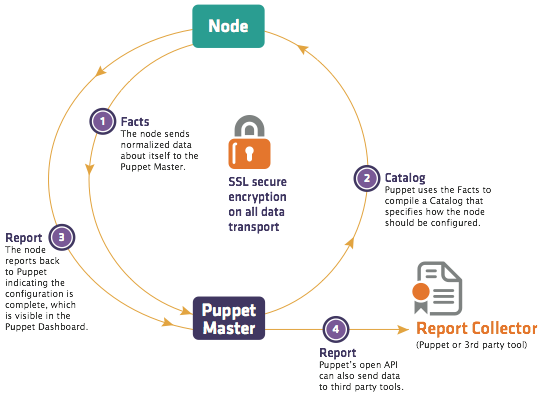
\includegraphics[width=13.5cm]{figuras/Puppet_Dataflow.png}
  \caption{Flujo de datos en Puppet.}
\label{figure:puppet-dataflow}
\end{figure}

Normalment Puppet se ejecuta de manera periódica mediante un planificador de trabajos (por ejemplo, cron). Cada cierto tiempo contactará con el nodo que debe ser administrado y volverá a repetir los pasos anteriores. Es decir, Puppet está continuamente intentando llevar al nodo al estado especificado en el manifiesto. Si entre una ejecución y otra algo cambiara en el nodo, Puppet se daría cuenta e intentaría llevar al nodo al estado especificado en el manifiesto.

Puppet, al igual que otras herramientas de configuración, trata de que los nodos converjan hacia un estado concreto, pero no garantiza que esto ocurra en una única ejecución. Es posible que sean necesarias varias ejecuciones de Puppet, aun cuando todo va bien, para alcanzar el estado deseado. Aunque esto pueda contrastar con la ejecución habitual de los programas, no es tan excepcional: si tenemos que poner en marcha dos servicios, de los cuales uno de ellos depende del otro, hasta que el primero no esté funcionando no podrá hacerlo el segundo. Una sola ejecución de Puppet no valdría para poner ambos servicios en marcha, sino que harían falta dos iteraciones como mínimo.
